\section{Lecture des acquisitions et premiers résultats}\label{sec:lecture-des-acquisitions-et-premiers-resultats}
   Maintenant que nous savons utiliser les récepteurs GNSS et enregistrer les mesures ainsi prises dans un fichier au format NMEA, vient désormais le moment de lire ces données avec Python afin de pouvoir les exploiter.

   \subsection{Implémentation}\label{subsec:implementation}
      Afin de rendre l'exploitation des données plus simple, plusieurs choix techniques ont été pris.
      Tout d'abord, la programmation en Python qui nous a paru adaptée à la forme du problème, le langage permettant facilement de traiter des données numériques contenues dans un fichier texte.

      Deuxièmement, il a été décidé de concevoir un programme orienté-objet, et donc d'implémenter une classe \texttt{Data} dans laquelle seront stockées les données contenues dans un fichier NMEA, ce qui permet alors, à partir d'une unique lecture des données du fichier d'acquisition, d'opérer différentes exploitations.
      Ainsi, il est possible à partir d'un simple fichier contenant des données NMEA d'instancier un objet \texttt{Data} qui en extraira l'ensemble des données à son initialisation.
      Il est alors possible d'opérer diverses opérations telles que le tracé d'un chemin GPS ou encore une étude métrologique comparative entre deux objets \texttt{Data} distincts, le tout en lisant une seule fois les données depuis le fichier texte.

      Nous allons donc, par la suite, détailler quelques opérations effectuées sur les données acquises.

   \subsection{Visualisation des données}\label{subsec:visualisation-des-donnees}
      \subsubsection{Nettoyage des données}
         Préalablement à la visualisation des données il est nécessaire de les \og nettoyer \fg{}, \ie transformer les données brutes du fichier texte en des données permettant essentiellement le transtypage des données numériques en entiers ou flottants.

         De plus, un problème rencontré avec les fichiers issus des relevés de terrain est la présence de certaines trames vides, ou encore des trames contenant des données incohérentes au milieu de données cohérentes.
         Il a donc été nécessaire, au moment de l'exploitation des données, de traiter ces cas.

         Pour le premier, une simple vérification des trames au moment de les extraire est suffisante : si les données \og essentielles \fg{} de la trame (typiquement la position et l'altitude) sont absentes, la trame est supprimée.
         Sont donc extraites pour visualisation et traitement uniquement les trames contenant des données exploitables.

         Pour le second, le principe de traitement est assez logique : lors de l'extraction de la position des trames NMEA, chaque couple de coordonnées est comparé au couple précédent.
         S'ils sont suffisamment proches (il est très improbable que le récepteur fasse un bond de position de l'ordre de la dizaine de kilomètres entre deux acquisitions successives), le couple de coordonnées est conservé.
         Sinon, il est considéré comme incohérent et est donc supprimé.

      \subsubsection{Visualisation 2D et 3D}
         Une fois les données exploitables, une première visualisation possible est, à partir des trames GGA (position du récepteur), l'évolution de la position du récepteur GNSS en deux dimensions (latitude et longitude).
         Ainsi, très simplement, les coordonnées extraites des trames GGA sont converties du format sexagésimal au format décimal afin d'être placées dans un repère 2D par le module \texttt{matplotlib} de Python, mais il est aussi possible de prendre en compte l'altitude, renseignée dans les trames GGA, pour obtenir un tracé en 3 dimensions.

         \begin{figure}[h]
             \centering
             \begin{subfigure}[h]{.45\textwidth}
                \centering
                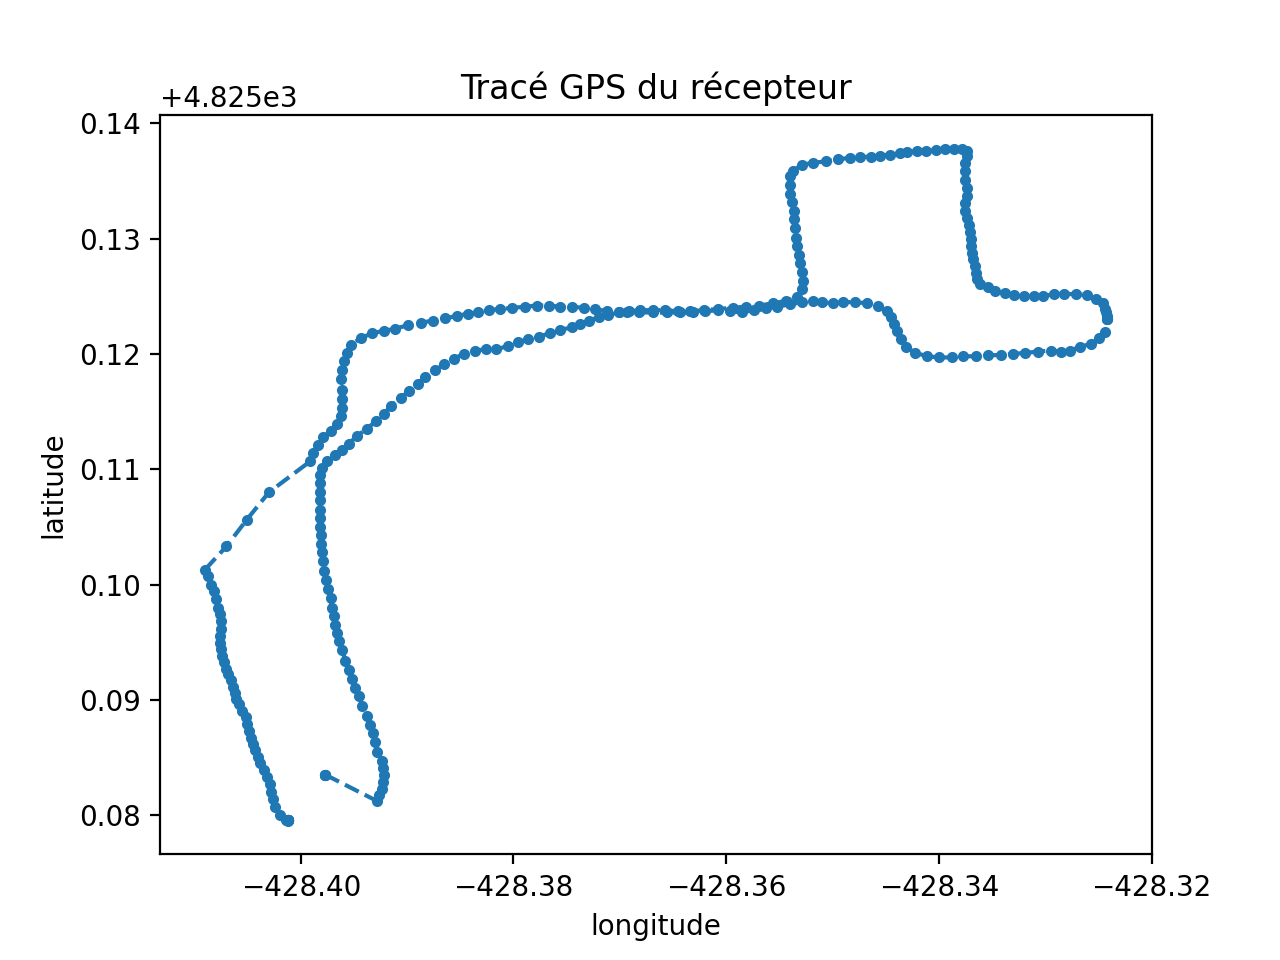
\includegraphics[width=\textwidth]{imgs/coords_2d}
             \end{subfigure}
             \hfill
             \begin{subfigure}[h]{.45\textwidth}
                \centering
                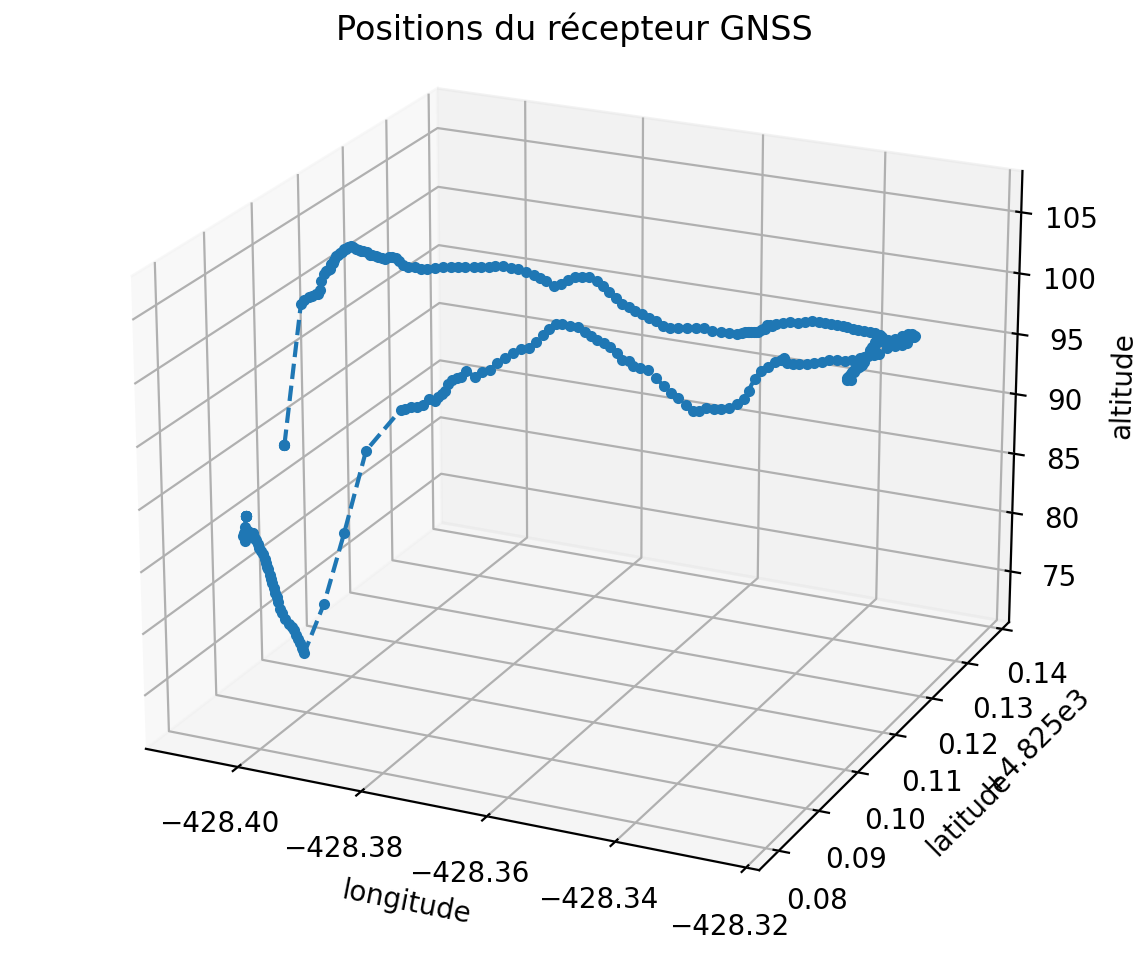
\includegraphics[width=\textwidth]{imgs/coords_3d}
             \end{subfigure}
             \caption{Position du récepteur en 2D et 3D}
             \label{fig:plot-coords}
         \end{figure}

      \subsubsection{Visualisation sur fond de carte}
         Bien que les représentations ainsi obtenues soient plutôt propres, elles ne sont pas très explicites pour l'utilisateur.
         Il serait alors intéressant de placer ces données sur un fond de carte afin d'obtenir une visualisation spatiale de la position du récepteur.

         Ce qui est permis en Python par le module \texttt{folium}, ayant des fonctionnalités de génération de carte au format HTML, en utilisant un fond de carte \textit{open-source} (\texttt{OpenStreetMap}) et transformant les coordonnées extraites des trames GGA en tracé grâce aux possibilités du format KML (permettant, au-dessus d'un fond de carte, d'afficher des figures géométriques telles que des points ou des lignes).

         \begin{figure}[h]
             \centering
             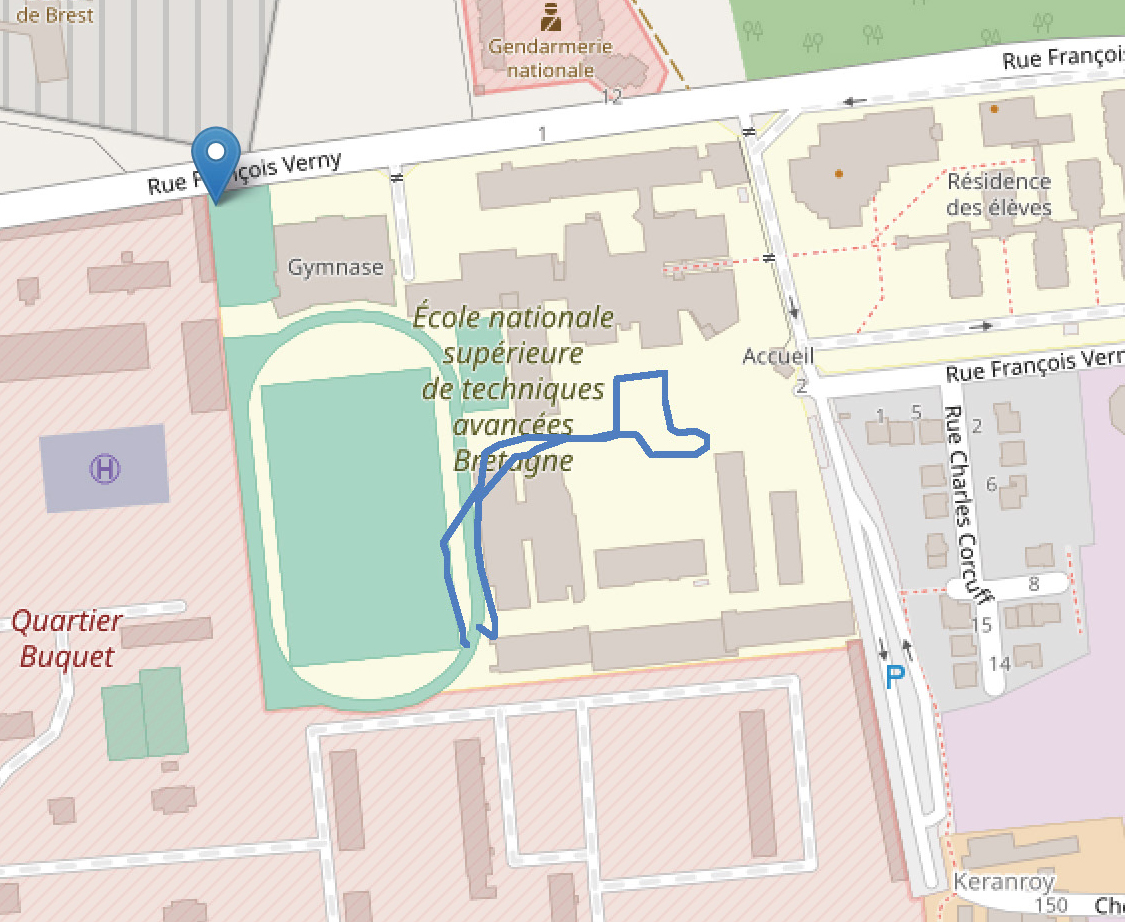
\includegraphics[width=.95\textwidth]{imgs/gps_map_2}
             \caption{Trace GPS sur un fond de carte HTML}
             \label{fig:coords-on-map}
         \end{figure}

         Le résultat est donc un fichier HTML contenant le tracé GPS extrait du fichier NMEA, superposé à un fond de carte manipulable par l'utilisateur.

         Les données mesurées sont donc, de cette manière, affichées à l'utilisateur de manière plus explicite et visuelle, lui permettant de voir les déplacements du récepteur au cours de l'acquisition.

         Une perspective intéressante serait également d'enregistrer les tracés de position non plus dans un fichier HTML avec un fond de carte, mais plutôt dans un fichier KML (format universel) pouvant être importé par exemple dans Google Earth afin que l'utilisateur puisse ajouter manuellement d'autres tracés à ces données acquises depuis un logiciel de visualisation d'informations géographiques.